\begin{appendices}

% \titleformat{\section}[display]
% {\normalfont\Large\bfseries}{\appendixname\enspace\thesection}{.5em}{}

\section{Additional Plots from Simulating Quantum Walk Entanglement Transfer}
\label{appendix:qw_figures}
\setcounter{figure}{0}
\renewcommand{\thefigure}{A.\arabic{figure}}
\begin{figure}[h]
    \centering
    $E_\mathcal{N}$\\
    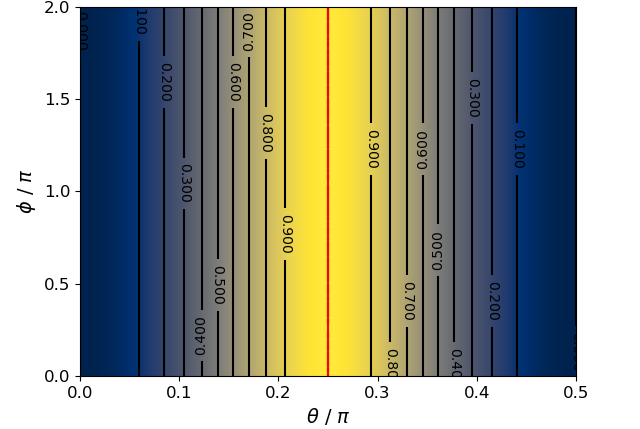
\includegraphics[width=0.9\textwidth]{1ebit_transfer.png}
    \caption{Log negativity of walkers after transferring entanglement from one Bell pair using the same projective measurements $\mathcal{P}_\gamma = \mathcal{P}_\delta$. This was simulated for 100 evenly spaced values of both $\theta$ and $\phi$. Every point along the red solid line has a peak value of 1.}
    \label{fig:1ebit_transfer}
\end{figure}

\begin{figure}
    \centering
    \medskip
    \begin{subfigure}{0.49\textwidth}
        \centering
        $E_\mathcal{N}$\\
        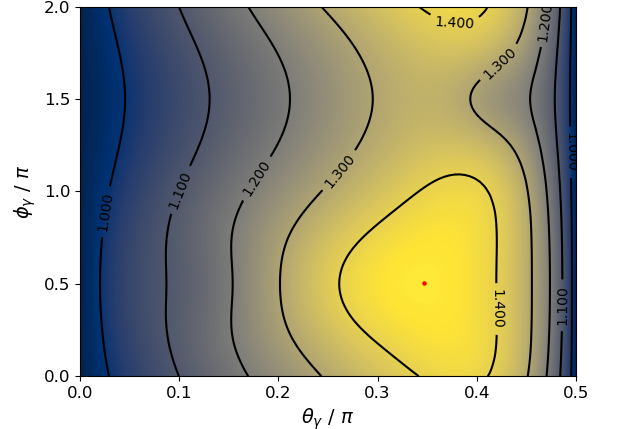
\includegraphics[width=\linewidth]{2ebit_transfer_fixed_0.125_0.5.png}
        \caption{$\theta_\delta = 0.125\pi$, $\phi_\delta = 0.5\pi$. Maximum $E_\mathcal{N}\sim 1.448$.}
    \end{subfigure}
    \hfill
    \begin{subfigure}{0.49\textwidth}
        \centering
        $E_\mathcal{N}$\\
        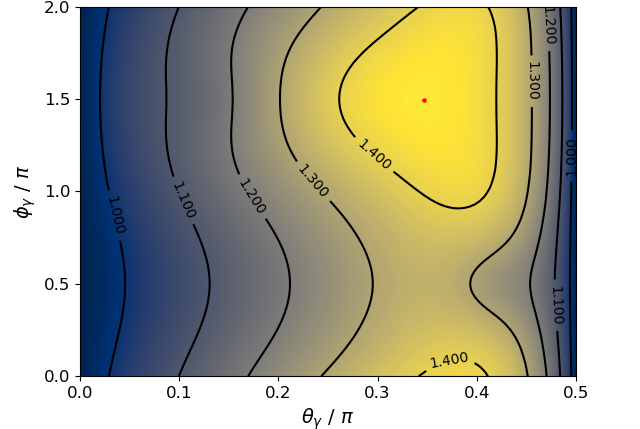
\includegraphics[width=\linewidth]{2ebit_transfer_fixed_0.125_1.5.png}
        \caption{$\theta_\delta = 0.125\pi$, $\phi_\delta = 1.5\pi$. Maximum $E_\mathcal{N}\sim 1.448$.}
    \end{subfigure}
    \par\medskip
    \begin{subfigure}{0.49\textwidth}
        \centering
        $E_\mathcal{N}$\\
        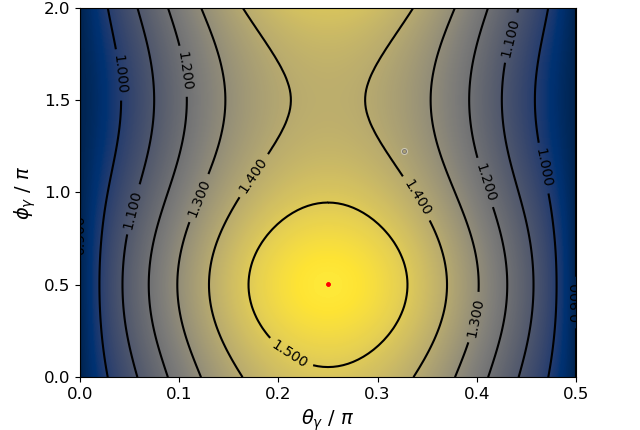
\includegraphics[width=\linewidth]{2ebit_transfer_fixed_0.25_0.5.png}
        \caption{$\theta_\delta = 0.25\pi$, $\phi_\delta = 0.5\pi$. Maximum $E_\mathcal{N}\sim 1.585$.}
    \end{subfigure}
    \hfill
    \begin{subfigure}{0.49\textwidth}
        \centering
        $E_\mathcal{N}$\\
        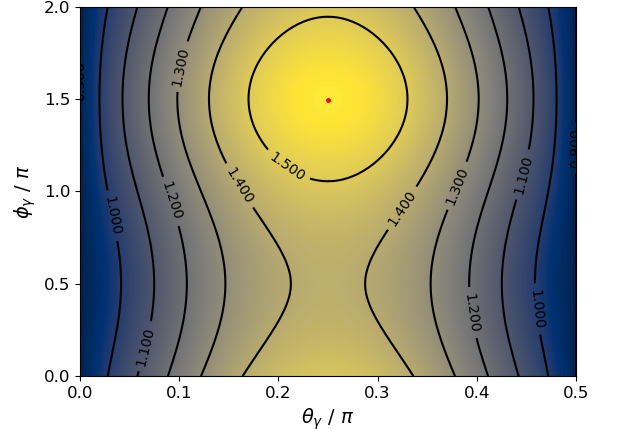
\includegraphics[width=\linewidth]{2ebit_transfer_fixed_0.25_1.5.png}
        \caption{$\theta_\delta = 0.25\pi$, $\phi_\delta = 1.5\pi$. Maximum $E_\mathcal{N}\sim 1.585$.}
    \end{subfigure}
    \par\medskip
    \begin{subfigure}{0.49\textwidth}
        \centering
        $E_\mathcal{N}$\\
        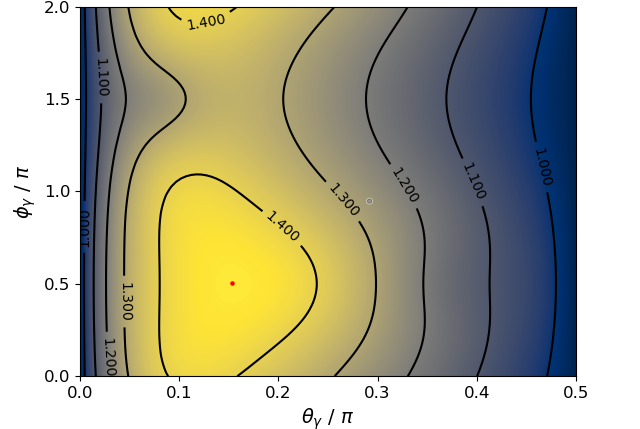
\includegraphics[width=\linewidth]{2ebit_transfer_fixed_0.375_0.5.png}
        \caption{$\theta_\delta = 0.375\pi$, $\phi_\delta = 0.5\pi$. Maximum $E_\mathcal{N}\sim 1.448$.}
    \end{subfigure}
    \begin{subfigure}{0.49\textwidth}
        \centering
        $E_\mathcal{N}$\\
        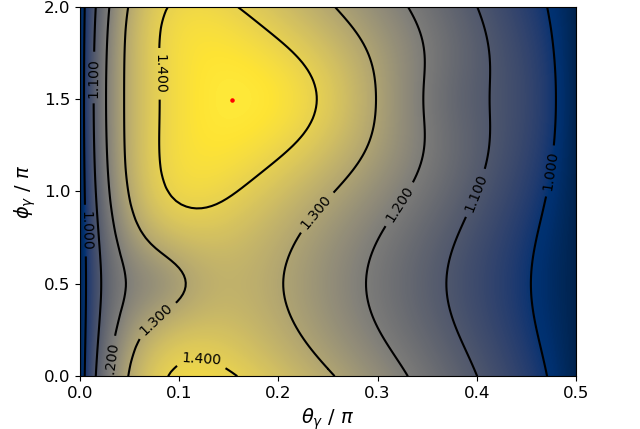
\includegraphics[width=\linewidth]{2ebit_transfer_fixed_0.375_1.5.png}
        \caption{$\theta_\delta = 0.375\pi$, $\phi_\delta = 1.5\pi$. Maximum $E_\mathcal{N}\sim 1.448$.}
    \end{subfigure}
    \caption{Plots showing the log negativity, $E_\mathcal{N}$, of walkers after transferring entanglement from two Bell pairs with different projective measurements $\mathcal{P}_\gamma \neq \mathcal{P}_\delta$. $\theta_\delta$, $\phi_\delta$ are fixed for $\mathcal{P}_\delta$, with the fixed values given in the captions. $\theta_\gamma, \phi_\gamma$ were each varied over 100 evenly spaced points for $\mathcal{P}_\gamma$. Peak values are indicated by red points.}
    \label{fig:2ebits_diff_proj}
\end{figure}

\newpage
\section{Proof of Claim \ref{claim:min_steps}}
\label{appendix:min_steps}
\setcounter{equation}{0}
\renewcommand{\theequation}{B.\arabic{equation}}
Here a proof is given for claim \ref{claim:min_steps}.

\begin{proof}
    Each step in a quantum walk with shift operator $\tilde{S}$ increases the number of basis states with non-zero amplitude by 1, provided that the amplitude $\ket{\downarrow}$ coin basis state is non-zero.
    Therefore the dimension of each walker can be taken to be $s + 1$, where $s$ is the total number of steps taken in the walk, since each walker space can be reduced to the subspace spanned by the $s+1$ non-zero amplitude basis states.
    Using claim \ref{claim:maximally_entangled_states}, the upper bound on the log negativity of the combined walker states after the $n^{\text{th}}$ iteration of the walk is given by $\log_2(s+1)$.
    This implies the following condition on the total number of steps
    \begin{equation}
        \log_2(s+1) = n \implies s = 2^n -1.
        \label{eqn:equality_on_s}
    \end{equation}
    This is an equality rather than an inequality $\log_2(s+1) \geq n$, since the state of the walkers is to be maximally entangled.
    This means that the combined walker Hilbert space $\mathcal{H}_W$ must be reducible to one of dimension $2^n \times 2^n$ (the same as the total dimension of the $n$ Bell pairs used for the protocol).
    This is only possible when taking the minimum number of steps in each quantum walk, if more steps are taken then there are more than $2^n$ basis states of non-zero amplitude for each walker.
    
    Let $s_{n-1}$ be the total number of steps taken up to the $(n-1)^\text{th}$ iteration of the protocol.
    If $s_{n-1}$ satisfies equation \ref{eqn:equality_on_s} this implies $s_{n-1} = 2^{n-1} -1$.
    Therefore, the number of steps for the $n^{\text{th}}$ iteration is given by
    \begin{align}
        s - s_{n-1} &= 2^{n} - 1 - (2^{n-1} -1)\\
        &= 2^n - 2^{n-1}\\
        &= 2 \times 2^{n-1} - 2^{n-1}\\
        &= 2^{n-1}.
    \end{align}
    For $n = 2$, it has been shown that $s_1 = 1$ therefore the claim is true by induction.
\end{proof}

\newpage
\section{Proof of Claim \ref{claim:COmegaCXinQFTbasis}}
\label{appendix:c_omega}
\setcounter{equation}{0}
\renewcommand{\theequation}{C.\arabic{equation}}

Here a proof is given for claim \ref{claim:COmegaCXinQFTbasis}.

\begin{proof}
    The Fourier basis state $\ket{+_k}_d$ is given by
    \begin{equation}
        \ket{+_k}_d = \frac{1}{\sqrt{d}}\sum_{m=0}^{d-1}\omega^{km}\ket{m}.
    \end{equation}
    Therefore
    \begin{align}
        C\text{-}\Omega^j\left(\ket{+_k}_d\ket{1}_2\right) 
        &= \frac{1}{\sqrt{d}}\sum_{m=0}^{d-1}C\text{-}\Omega^j\left(\omega^{km}\ket{m}_d\otimes\ket{1}_2\right)\\
        &= \frac{1}{\sqrt{d}}\sum_{m=0}^{d-1}\omega^{mj}\left(\omega^{km}\ket{m}_d\otimes\ket{1}_2\right)\\
        &= \frac{1}{\sqrt{d}}\sum_{m=0}^{d-1}\omega^{(k+j)m}\ket{m}_d\otimes\ket{1}_2\\
        &= \left(\frac{1}{\sqrt{d}}\sum_{m=0}^{d-1}\omega^{(k+j)m}\ket{m}_d\right)\otimes\ket{1}_2\\
        &= \ket{+_{k+j}}_d\otimes\ket{1}_2.
    \end{align}
\end{proof}

\newpage
\section{Proof that the AQC Circuit Can Store Any Number of Qubits}
\setcounter{equation}{0}
\renewcommand{\theequation}{D.\arabic{equation}}
\label{appendix:any_num_qubits}
Here it is proven by induction that the circuit presented in section \ref{section:furtheruses} can store $n\in\mathbb{N}$ qubit states into the qudit, as long as the dimension of the Hilbert space $d\geq 2^n$.
\begin{proof}$ $\newline
    $n=1$\newline
    It has already been shown in equation \ref{eqn:single_qbit_store} that a single arbitrary qubit state can be stored giving
    \begin{equation}
        (a_1\ket{0}_d + b_1\ket{1}_d)\otimes\ket{0}_2,
    \end{equation}
    where the coefficients have been relabelled $a \rightarrow a_1, b\rightarrow b_1$.
    \newline

    $n = k$\newline
    Assume that $n$ qubit states have been stored in the qudit, giving the qudit state
    \begin{equation}
        \left(\sum_{j=0}^{2^k - 1}c_j\ket{j}_d\right)\otimes\ket{0}_2.
        \label{eqn:sum_qudit_state}
    \end{equation}
    Furthermore, assume that this can be re-expressed as a tensor product of $n$ qubits by converting the computational basis state labels to their binary equivalents and "expanding" to give
    \begin{align}
        &(a_k\ket{0} + b_k\ket{1})\otimes(a_{k-1}\ket{0} + b_{k-1}\ket{1})\otimes\cdots\otimes(a_1\ket{0} + b_1\ket{1})\otimes\ket{0}_2\\
        &=\bigotimes_{i = k}^{1}\left(a_i\ket{0} + b_i\ket{1}\right)\otimes\ket{0}_2,
    \end{align}
    where the coefficients $a_{i}$ and $b_{i}$ match the amplitudes of the $i^{\text{th}}$ qubit state that was stored.
    Note that the assumption that the state can be expanded in such a way implies equation \ref{eqn:sum_qudit_state} where
    \begin{equation}
        c_j = \prod_{i=1}^{k}(a_i \delta^{0}_{j_{2_i}} + b_i\delta^{1}_{j_{2_i}}),
    \end{equation}
    where $j_{2_i}$ is the $i^{\text{th}}$ digit of the binary expression of $j$, and $\delta^m_n$ is the Kronecker delta.\newline
    \newpage

    $n=k+1$\newline
    The entire state prior to running the circuit with an additional qubit to be stored is given by
    \begin{align}
        &\left(\bigotimes_{i = k}^{1}(a_i\ket{0} + b_i\ket{1})\right)\otimes(a_{k+1}\ket{0}_2 + b_{k+1}\ket{1}_2)\\
        =&\left(\bigotimes_{i = k}^{1}(a_i\ket{0} + b_i\ket{1})\right)\otimes a_{k+1}\ket{0}_2\label{eqn:sum_state}
        +
        \left(\bigotimes_{i = k}^{1}(a_i\ket{0} + b_i\ket{1})\right)\otimes b_{k+1}\ket{1}_2.
    \end{align}
    This state is now put through the circuit.
    Note that the summand which is tensored with $\ket{0}_2$ is not affected by the $\C{\Omega^j}$ since the target is $\ket{0}_2$.
    Therefore only the summand tensored with $\ket{1}_2$ is advanced, and by claim \ref{claim:COmegaCXinQFTbasis}, the basis states are shifted up by $j$ steps.
    From claim \ref{claim:min_steps}, for the $\C{\Omega^j}$ gate, $j = 2^k$.
    Consider what this means in terms of computational basis states.
    When written in terms of computational basis states, equation \ref{eqn:sum_state} is given by the sum
    \begin{align}
        &\left(\sum_{i=0}^{2^k - 1}c_i\ket{i}_d\right) \otimes a_{k+1}\ket{0}_2
        +\left(\sum_{i=0}^{2^k - 1}c_i\ket{i}_d\right) \otimes b_{k+1}\ket{1}_2.
    \end{align}
    Shifting all of the computational basis states in the second summand by $j=2^k$ yields
    \begin{align}
        \left(\sum_{i=0}^{2^k - 1}c_i\ket{i}_d\right) \otimes a_{k+1}\ket{0}_2
        +\left(\sum_{i=0}^{2^k - 1}c_i\ket{i + 2^k}_d\right) \otimes b_{k+1}\ket{1}_2.
    \end{align}
    In binary, adding $2^k$ to a number that is less than $2^k$ can be thought of as placing an additional 1 at the start of the string of binary digits.
    For example, where $(x)_2$ denotes that the number $x$ is written in binary,
    \begin{equation}
        7 + 8 = (2^3 - 1) + (2^3) = (111)_2 + (1000)_2 = (1111)_2.
    \end{equation}
    In this way, the action of the $\C{\Omega^j}$ gate on the tensor representation of the qudit given in equation \ref{eqn:sum_state} can be thought of as adding a $\ket{1}$ in front of all of the binary representations of the computational basis states tensored with $\ket{1}_2$.
    Similarly, a $\ket{0}$ can be added in front of the binary representations of the computational basis states tensored with $\ket{0}_2$, since it still represents the same number ($01 = 1$).
    \begin{align}
        &\ket{0} \otimes \left(\bigotimes_{i = k}^{1}(a_i\ket{0} + b_i\ket{1})\right)\otimes a_{k+1}\ket{0}_2
        +
        \ket{1} \otimes \left(\bigotimes_{i = k}^{1}(a_i\ket{0} + b_i\ket{1})\right)\otimes b_{k+1}\ket{1}_2\\
        =&a_{k+1}\ket{0} \otimes \left(\bigotimes_{i = k}^{1}(a_i\ket{0} + b_i\ket{1})\right)\otimes \ket{0}_2
        +
        b_{k+1} \ket{1} \otimes \left(\bigotimes_{i = k}^{1}(a_i\ket{0} + b_i\ket{1})\right)\otimes \ket{1}_2.
    \end{align}
    It is only possible to add these additional kets if the $d \geq 2^{k+1}$, else the Hilbert space is not large enough to accommodate the additional states being represented, hence the need for that constraint.
    The next step of the circuit is to use some map $U$ to pair the even numbered computational basis states with $\ket{0}_2$ and the odd numbered computational basis states with $\ket{1}_2$ to convert the $\ket{1}_2$ to a $\ket{0}_2$ via a $\C{X}$ operation, after which $U$ is uncomputed.
    On the qudit state, since no amplitude changes are involved, this is akin to doing a $UU^{-1}=I$ and so leaves the qudit state untouched.
    Therefore the final state is given by
    \begin{align}
        &a_{k+1}\ket{0} \otimes \left(\bigotimes_{i = k}^{1}(a_i\ket{0} + b_i\ket{1})\right)\otimes \ket{0}_2
        +
        b_{k+1} \ket{1} \otimes \left(\bigotimes_{i = k}^{1}(a_i\ket{0} + b_i\ket{1})\right)\otimes \ket{0}_2\\
        =&\left(a_{k+1}\ket{0}+b_{k+1} \ket{1}\right) \otimes \left(\bigotimes_{i = k}^{1}(a_i\ket{0} + b_i\ket{1})\right)\otimes \ket{0}_2\\
        =&\left(\bigotimes_{i = k+1}^{1}(a_i\ket{0} + b_i\ket{1})\right)\otimes \ket{0}_2.
    \end{align}
    So the statement is true by induction.
\end{proof}
\end{appendices}